\chapter{Related Work\label{cha:chapter5}}

\hspace*{1em}
\begin{figure}[b!]
    \centering
    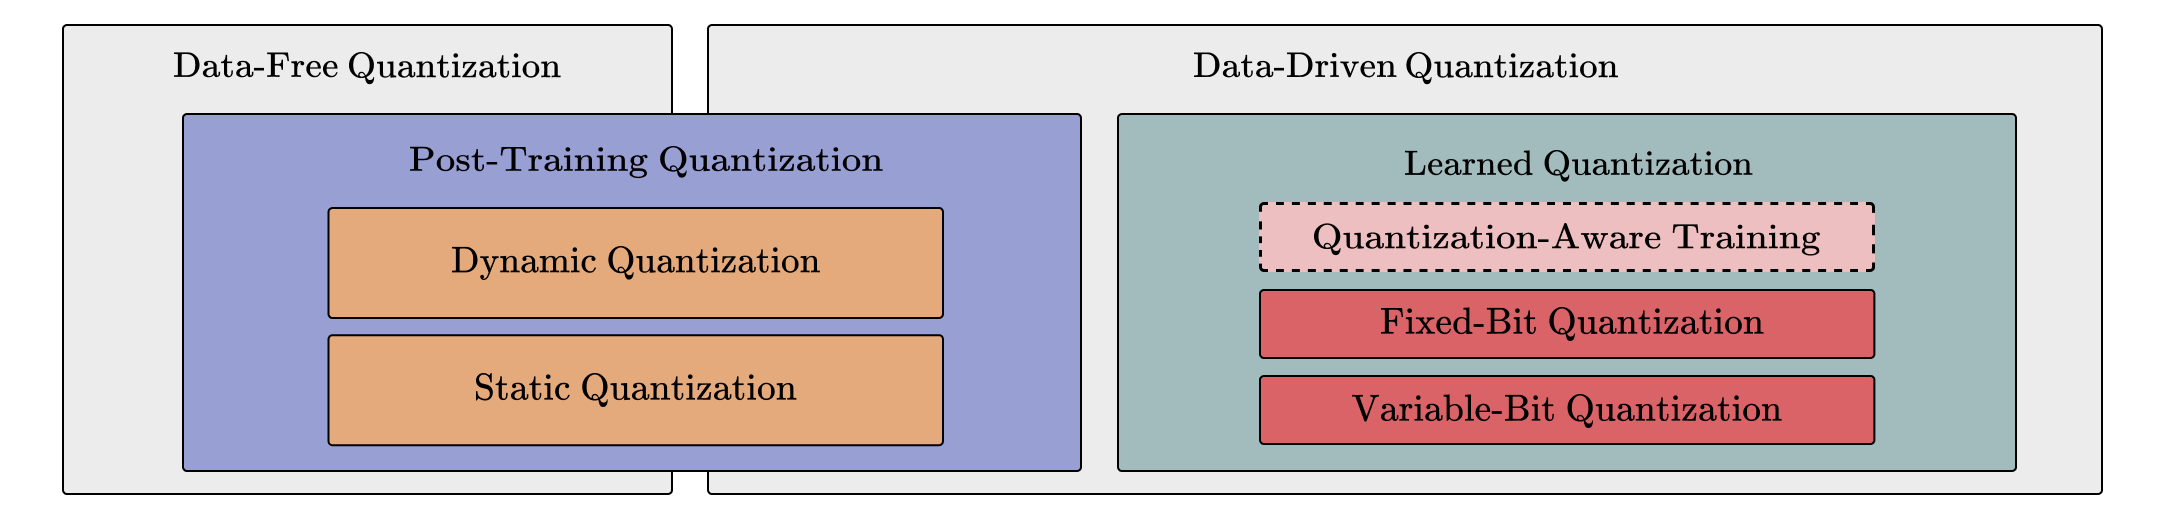
\includegraphics[width=14cm]{related_work.png}
    \caption{ Learned quantization in a broader context.}
    \label{fig:related_work}
  \end{figure}
  
The hyperparameter space of deep neural networks is so vast
that classifying research in the field of learned quantization into rigid groups
is inherently challenging.
Nevertheless, we aim to outline a rough distinction
between different approaches by emphasizing their most apparent aspects,
after first establishing the position of learned quantization within the broader field of quantization.

\textbf{Data-Free vs. Data-Driven Quantization.}
As discussed in \cref{cha:chapter2}, 
data-free quantization relies solely on the intrinsic properties of ML models, 
such as weight distribution statistics, to determine quantization parameters \cite{DBLP:conf/iccv/NagelBBW19}. 
In contrast, data-driven quantization uses the original training data to fine-tune the model to the quantization strategy \cite{Edouard2022SPIQ}. 
Although learned quantization does not strictly align with the definition of a fine-tuning process, 
it incorporates the full training pipeline, jointly optimizing both the model and the quantization parameters. 
This characteristic makes it inherently data-driven. 
Thus, we regard learned quantization as a distinct subcategory within data-driven quantization approaches.

\textbf{PTQ vs. QAT.}
PTQ \cite{DBLP:conf/icmcs/ZhuZL18} can fall into either the data-free or data-driven category, depending on the parameters being quantized. 
If it’s just weights, it’s data-free since weights can be quantized without relying on input data. 
However, if activations are included, it’s data-driven because activation quantization needs input data for calibration. 
Since PTQ doesn’t involve training on the full dataset, it’s distinct from learned quantization.
QAT, on the other hand, does involve full training, where the model adapts to the quantization strategy. 
This makes it part of learned quantization, which may also involve learning the quantization parameters themselves as part of the process.

\textbf{Static vs. Dynamic Quantization.} 
Static quantization is an offline method that quantizes weights and activations before inference, 
whereas dynamic quantization is applied on-the-fly during inference. 
Both static and dynamic quantization methods are post-training approaches. 
In the context of learned quantization, 
static quantization might refer to a fixed quantization scheme, 
and dynamic quantization  — to a scheme 
that depends on trainable quantizers.
However, these terms are not commonly used this way in the literature.
Therefore, we consider static and dynamic quantization separately from learned quantization. 

Having established the broader context of quantization, 
we will now attempt to classify the various approaches within learned quantization itself.

\textbf{Fixed-Bit vs. Variable-Bit.} 
Learned quantization schemes can be roughly divided into two broader groups. 
The first group involves quantization schemes that use a fixed target bit size, 
while the second group aims to learn or effectively determine the lowest feasible bit size. 
This distinction is not widely discussed in the literature, 
but we view it as a recognizable pattern. 
For example, LQ-Nets \cite{DBLP:conf/eccv/ZhangYYH18} compute binary encodings of model parameters using a predefined bit size, 
whereas LSQ \cite{DBLP:conf/iclr/EsserMBAM20} learns step sizes in a way that can adaptively reduce bit width requirements.

\textbf{Quantization Target.} NNs offer multiple opportunities for applying quantization.
While some learned quantization approaches focus exclusively on model weights \cite{polino2018modelcompression} \cite{ott2016rnn} \cite{courbariaux2015binaryconnect} \cite{DBLP:journals/pnas/EsserMACAABMMBN16},
others extend this to include activations \cite{krishnamoorthi2018quantizing} \cite{hubara2016qnn} \cite{rastegari2016xnor} \cite{Edouard2022SPIQ} \cite{DBLP:conf/eccv/ZhangYYH18}
and even gradients \cite{DBLP:journals/corr/LinCMB15} \cite{DBLP:conf/icml/Zhang0KALZ17}. As notable examples,
DoReFa-Net \cite{shuchang2016dorafenet} quantizes all three with arbitraty bitwidths, 
whereas Quantized Neural Networks \cite{hubara2016qnn} constrain weights and activations to either 
\( -1 \) or \( +1 \), and quantize gradients to \( 6 \) bits.

\textbf{Quantization Precision.}
The target lower bit precision, and whether it is adjustable, 
varies between methods — ranging from rigid constraints to only a few values, 
to the flexibility of setting the desired bitwidth. 
For instance, BinaryNet \cite{DBLP:conf/nips/HubaraCSEB16} and XNOR-Net \cite{rastegari2016xnor} 
represent extreme cases of quantization, 
where weights and activations are binarized. 
Ternary Weight Networks \cite{DBLP:conf/icassp/LiuLWZY23} take a slightly less aggressive approach 
by quantizing weights to \( -1, 0, 1 \). 
In contrast, DoReFa-Net \cite{shuchang2016dorafenet} allows the target bit size to be defined.

\textbf{Quantization Granularity.} 
Learned quantization methods differ in how granularly the quantization is applied, 
that is, the level of detail at which model parameters are quantized. 
To illustrate, Benoit et al. \cite{jacob2018quantization} implement layer-wise quantization  — 
similar to QIL \cite{DBLP:conf/cvpr/JungSLSHKHC19} and PACT \cite{DBLP:journals/corr/abs-1805-06085}  — 
whereas LQ-Nets \cite{DBLP:conf/eccv/ZhangYYH18} employ channel-wise quantization for weights, 
despite using layer-wise quantization for activations.

\textbf{Combination with Other Techniques.} 
A number of learned quantization methods work in unison with other model compression approaches.
For example, Deep Compression \cite{han2016deepcompression} combines quantization with pruning, while 
Polino et al. \cite{polino2018modelcompression} and Wei et al. \cite{DBLP:conf/eccv/WeiPQOY18} 
jointly leverage quantization and knowledge distillation.

To summarize, the landscape of learned quantization is as diverse as it gets.
While the classifications outlined in this chapter are by no means exhaustive, 
they represent those we find most apparent and distinguishable.
Together with \cref{cha:chapter2}, 
this chapter aims to provide a broader pitcture of learned quantization. 
Building on this picture,
we will reflect on the contributions of this thesis and outline potential directions for future research in the conclusion.
